\chapter{Comparing distributions}
\label{ch:comparingdistributions}

The previous chapters have introduced a plethora of parametric
distributions that allow us to test hypotheses and assess the
precision of experimental results. However these inferences are only
as strong as the assumptions on which they are based.  For example,
Chapter~\ref{ch:binomial} used a binomial distribution to assess the
occurrence of gold in a prospecting area, assuming that the gold was
randomly distributed across all the claims; and
Chapter~\ref{ch:poisson} used a Poisson distribution to model
earthquakes, assuming that the earthquake catalog was free of clusters
and that all aftershocks had been removed from it. This chapter will
introduce some strategies to test these assumptions, both graphically
and numerically.

\section{Q-Q plots}
\label{sec:q-q}

As the name suggests, a quantile-quantile or Q-Q plot is a graphical
method for comparing two probability distributions by plotting their
quantiles against each other. Q-Q plots set out the quantiles of a
sample against those of a theoretical distribution, or against the
quantiles of another sample. For example, comparing the Old Faithful
eruption duration dataset (Figure~\ref{fig:CLTfaithful1}) to a normal
distribution:

\noindent\begin{minipage}[t][][b]{.3\textwidth}
  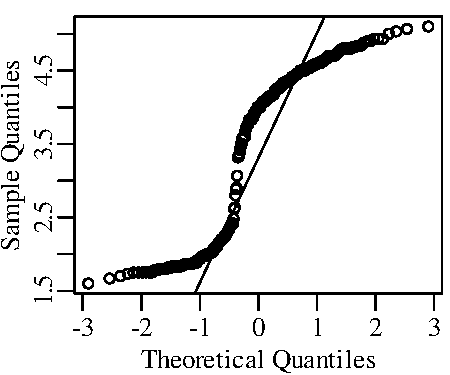
\includegraphics[width=\textwidth]{../figures/qqfaithful1.pdf}\medskip
\end{minipage}
\begin{minipage}[t][][t]{.7\textwidth}
  \captionof{figure}{Quantile-quantile (Q-Q) plot of Old Faithful
    eruption durations. The horizontal axis marks the theoretical
    quantiles of a normal distribution with the same mean and standard
    deviation as the data. The vertical axis marks the quantiles of
    the actual data. If the two distributions being compared are
    similar, the points in the Q-Q plot will approximately lie on the
    line y = x. Otherwise they will not. In this example the
    distribution of eruption durations clearly does not follow a
    normal distribution.}
  \label{fig:qqfaithful1}
\end{minipage}

\noindent\begin{minipage}[t][][b]{.3\textwidth}
  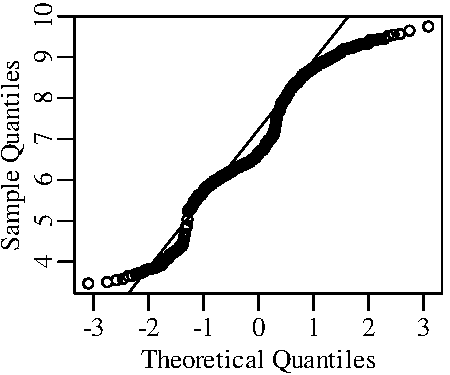
\includegraphics[width=\textwidth]{../figures/qqfaithful2.pdf}\medskip
\end{minipage}
\begin{minipage}[t][][t]{.7\textwidth}
  \captionof{figure}{Q-Q plot of the dataset of 500 sums of $n = 2$
    randomly selected eruption durations shown in
    Figure~\ref{fig:CLTfaithful2}. The resulting trimodal distribution
    plots closer to the 1:1 line than the original dataset of
    Figure~\ref{fig:qqfaithful1} but is still far from normal.}
  \label{fig:qqfaithful2}
\end{minipage}

\noindent\begin{minipage}[t][][b]{.3\textwidth}
  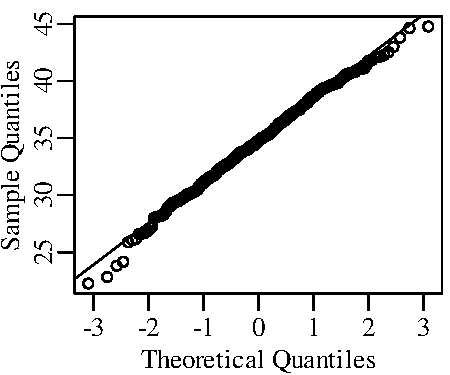
\includegraphics[width=\textwidth]{../figures/qqfaithful10.pdf}\medskip
\end{minipage}
\begin{minipage}[t][][t]{.7\textwidth}
  \captionof{figure}{Q-Q plot of the dataset of 500 sums of $n = 10$
    randomly selected eruption durations shown in
    Figure~\ref{fig:CLTfaithful10}. The data plot very close to the
    1:1 line, visually confirming that they follow a normal
    distribution.  The sample distribution only deviates from the
    theoretical distribution at the most extreme quantiles. This
    indicates that the sample distribution has heavier tails than the
    normal distribution. This phenomenon will be discussed further in
    the next section. Increasing $n$ further would remove this effect
    near the tails and bring the sample distribution even closer to
    the normal distribution.}
  \label{fig:qqfaithful10}
\end{minipage}

Q-Q plots cannot only be used to compare sample distributions with
theoretically predicted parametric distributions, but also to compare
one sample with another. For example:

\noindent\begin{minipage}[t][][b]{.3\textwidth}
  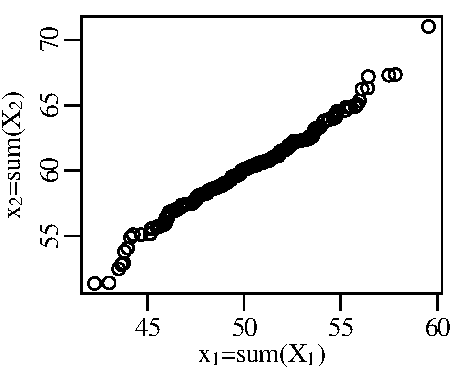
\includegraphics[width=\textwidth]{../figures/qqfaithful12.pdf}\medskip
\end{minipage}
\begin{minipage}[t][][t]{.7\textwidth}
  \captionof{figure}{ Q-Q plot comparing datasets
    $x_1=\mbox{sum}(X_1)$ and $x_2=\mbox{sum}(X_2)$ of
    Figure~\ref{fig:rand2sum}. Even though the two datasets have
    markedly different means ($\bar{x}_1=50.0$ and $\bar{x}_2=59.9$)
    and slightly different standard deviations ($s[x_1]=3.3$ and
    $s[x_2]=3.1$), the quantiles of the two datasets plot along a
    straight line. This means that their distributions are identical
    in shape.  }
  \label{fig:qqfaithful12}
\end{minipage}

\section{The t-test}
\label{sec:t}

The Q-Q plot in Figure~\ref{fig:qqfaithful12} compared two samples
that were normally distributed with different means.  However it may
not be clear if the difference between the means is statistically
significant or not. Before we address this problem, let us first look
at a related but slightly simpler problem. Consider the density of 5
gold coins as an example:

\begin{center}
\begin{tabular}{c|ccccc}
  coin \# & 1 & 2 & 3 & 4 & 5 \\ \hline
  density (g/cm\textsuperscript{3}) & 19.09 & 19.17 & 19.31 & 19.07 & 19.18
  \label{tab:coins}
\end{tabular}
\end{center}

The density of pure gold is 19.30~g/cm\textsuperscript{3}. We might
ask ourselves the question if the five coins are made of pure gold, or
if they consist of an allow that mixes gold with a less dense metal?
To answer this question, we assume that the sample mean $\bar{x}$
follows a normal distribution with mean $\mu$ and standard deviation
$\sigma/\sqrt{n}$ (following the same derivation as
Equation~\ref{eq:stderrmean}). Thus, the parameter
\begin{equation}
  z = \frac{\bar{x}-\mu}{\sigma/\sqrt{n}}
  \label{eq:z}
\end{equation}

\noindent follows a \textbf{standard normal distribution} whose mean
is zero and whose standard deviation is one. As we have seen in
Section~\ref{sec:normalparameters}, $\sigma$ is unknown but can be
estimated by the sample standard deviation $s[x]$. We can then
replace Equation~\ref{eq:z} with a new parameter
\begin{equation}
  t = \frac{\bar{x}-\mu}{s[x]/\sqrt{n}}
  \label{eq:t}
\end{equation}

However $t$ does not follow a normal distribution but a
\textbf{Student t-distribution} with $(n-1)$ \textbf{degrees of
  freedom} where the $(n-1)$ plays a similar role as the Bessel
correction of Section~\ref{sec:normalparameters}. It accounts for the
`double use' of the data to estimate both the mean and the standard
deviation of the data. The t-distribution forms the basis of a
statistical test that follows the same sequence of steps as in
Sections~\ref{sec:binomH} and \ref{sec:poishyp}.

\begin{enumerate}
\item  Formulate two hypotheses:\medskip

  \noindent\begin{minipage}{.4\textwidth}
    $H_0$ (\textbf{null hypothesis})
    
    \vspace{1em}
    
    $H_{\!A}$ (\textbf{alternative hypothesis}):
  \end{minipage}
  \begin{minipage}{.2\textwidth}
  \end{minipage}
  \begin{minipage}{.2\textwidth}
    $\mu=19.30$
    
    \vspace{1em}
    
    $\mu<{19.30}$
  \end{minipage}
  \begin{minipage}{.2\textwidth}
  \end{minipage}
  
\item Calculate the following test statistic:

  \begin{equation}
    t = \frac{\bar{x} - \mu_\circ}{s[x]/\sqrt{n}}
    \label{eq:t1}
  \end{equation}

  \noindent where $\bar{x} = 19.164$, $\mu_\circ = 19.30$, 
  $s[x] = 0.0948$, and $n = 5$ so that $t = -3.2091$.

\item Under $H_0$, Equation~\ref{eq:t1} follows a Student
  t-distribution with 4 degrees of freedom. Tabulating some key
  quantiles of this distribution:

  \begin{center}
    \begin{tabular}{c|c@{\gap}c@{\gap}c@{\gap}c@{\gap}
        c@{\gap}c@{\gap}c@{\gap}c@{\gap}c@{\gap}c@{\gap}c@{\gap}c}
      $t$ & -3.75 & \textit{-3.2091} & -2.78 & -2.13 & -1.53 & -0.74 &
      0 & 0.74 & 1.53 & 2.13 & 2.78 & 3.75 \\ \hline
      $P(T\leq{t})$ & 0.01 & \textit{0.0163} & 0.025 & 0.05 & 0.1 & 0.25 &
      0.5 & 0.75 & 0.9 & 0.95 & 0.975 & 0.99
    \end{tabular}
  \end{center}

  \noindent where the observed value is marked in italics.
  
\item We will use the usual confidence level $\alpha = 0.05$.

\item Marking the rejection region ($P(T<t)<\alpha$) in bold:
  
  \begin{center}
    \begin{tabular}{c|c@{\gap}c@{\gap}c@{\gap}c@{\gap}
        c@{\gap}c@{\gap}c@{\gap}c@{\gap}c@{\gap}c@{\gap}c@{\gap}c}
      $t$ & \textbf{\textit{-3.75}} & \textbf{\emph{-3.2091}} & \textbf{-2.78} &
      \textbf{-2.13} & -1.53 & -0.74 & 0 & 0.74 & 1.53 & 2.13 & 2.78 & 3.75 \\ \hline
      $P(T\leq{t})$ & \textbf{0.01} & \textbf{\textit{0.0163}} & \textbf{0.025} &
      \textbf{0.05} & 0.1 & 0.25 & 0.5 & 0.75 & 0.9 &
      0.95 & 0.975 & 0.99
    \end{tabular}
  \end{center}

  The one-sided rejection region consists of all $t<-2.10$.

\item Because the observed value of $t=-3.2091$ falls inside the
  rejection region, the null hypothesis is rejected.

\end{enumerate}

We therefore conclude that the coins are not made of pure gold. Here
is a graphical representation of this test:

\noindent\begin{minipage}[t][][b]{.6\textwidth}
  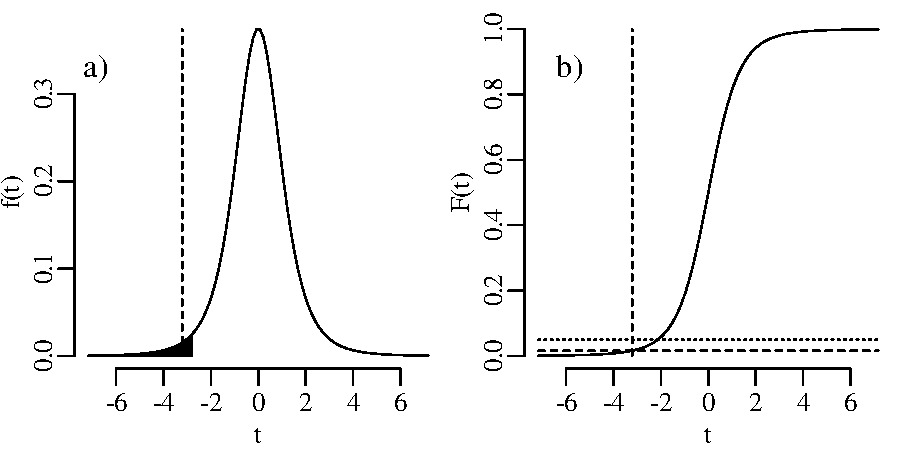
\includegraphics[width=\textwidth]{../figures/1samplettest.pdf}\medskip
\end{minipage}
\begin{minipage}[t][][t]{.4\textwidth}
  \captionof{figure}{a) PDF and b) CDF of a t-distribution with 4
    degrees of freedom. The one-sided rejection region (for
    $\alpha=0.05$) is marked in black. The vertical dashed line marks
    the observed value of $t=-3.2091$. This line plots in the
    rejection region, leading to the conclusion that
    $\mu<{19.30}$~g/cm\textsuperscript{3}. The horizontal dashed line
    marks the p-value ($0.0163<\alpha$).}
  \label{fig:1samplettest}
\end{minipage}

The comparison between the mean of a sample (coin densities) and a
particular value (19.30~g/cm\textsuperscript{3}) is called a
\textbf{one sample t-test}. If we want to compare the mean densities
of two samples, then that would require a \textbf{two sample
  t-test}. For example, consider the following two collections of
coins:

\begin{center}
\begin{tabular}{c|ccccc}
  coin \# & 1 & 2 & 3 & 4 & 5 \\ \hline
  density (1\textsuperscript{st} collection) &
  19.09 & 19.17 & 19.31 & 19.07 & 19.18 \\
  density (2\textsuperscript{nd} collection) &
  19.30 & 19.33 & 19.15 & 19.32
  \label{tab:2setcoins}
\end{tabular}
\end{center}

The average densities of collection~1 and 2 are 19.164~g/cm$^3$ and
19.275~g/cm$^3$, respectively. If we assume that the two collections
have the \textit{same variance}, then we can test whether the
difference between the two means is significant or not.

\begin{enumerate}
\item  Formulate two hypotheses:\medskip

  \noindent\begin{minipage}{.4\textwidth}
    $H_0$ (\textbf{null hypothesis})
    
    \vspace{1em}
    
    $H_{\!A}$ (\textbf{alternative hypothesis}):
  \end{minipage}
  \begin{minipage}{.2\textwidth}
  \end{minipage}
  \begin{minipage}{.2\textwidth}
    $\mu_1=\mu_2$
    
    \vspace{1em}
    
    $\mu_1\neq{\mu_2}$
  \end{minipage}
  \begin{minipage}{.2\textwidth}
  \end{minipage}
  
\item Calculate the following test statistic:
  \begin{equation}
    t = \frac{\bar{x}_1 - \bar{x}_2}{s_p\sqrt{\frac{1}{n_1}+\frac{1}{n_2}}}
    \label{eq:t2}
  \end{equation}

  \noindent where $\bar{x}_1 = 19.164$, $n_1 = 5$, $\bar{x}_2 =
  19.275$, $n_2 = 4$, and $s_p$ is the \emph{pooled} standard
  deviation:
  \begin{equation}
    s_p = \sqrt{\frac{(n_1-1) s[x_1]^2 + (n_2-1) s[x_2]^2}{n_1 + n_2 - 2}}
    \label{eq:sp}
  \end{equation}

  \noindent in which $s[x_1]=0.095$ and $s[x_2]=0.084$ are the
  standard deviations of the first and second coin collection,
  respectively. Plugging the data into equations \ref{eq:t2} and
  \ref{eq:sp} yields $t=-1.857$.

\item Under $H_0$, Equation~\ref{eq:t2} follows a Student
  t-distribution with $(n_1+n_2-2)$ degrees of freedom\footnote{Two
    degrees of freedom have been removed because we estimated two
    parameters from the data: $\bar{x}_1$ and
    $\bar{x}_2$.}. Tabulating some key quantiles of the t-distribution
  with 7 degrees of freedom:

  \begin{center}
    \begin{tabular}{c|c@{\gap}c@{\gap}c@{\gap}c@{\gap}
        c@{\gap}c@{\gap}c@{\gap}c@{\gap}c@{\gap}c@{\gap}c@{\gap}c}
      $t$ & -3.00 & -2.36 & -1.89 & \textit{-1.857} & -1.41 & -0.71 &
      0.00 & 0.71 & 1.41 & 1.89 & 2.36 & 3.00 \\ \hline
      $P(T\leq{t})$ & 0.01 & 0.025 & 0.05 & \textit{0.053} & 0.1 & 0.25 &
      0.5 & 0.75 & 0.9 & 0.95 & 0.975 & 0.99 \\
      $P(T\geq{t})$ & 0.99 & 0.975 & 0.95 & \textit{0.947} & 0.9 & 0.75 & 0.5 &
      0.25 & 0.1 & 0.05 & 0.025 & 0.01
    \end{tabular}
  \end{center}
  
  \noindent where the observed value is marked in italics.
  
\item We will use the conventional confidence level $\alpha =
  0.05$. But because we are carrying out a two-sided test, we will
  have two cutoff regions marked by $\alpha/2$ and $(1-\alpha/2)$,
  respectively.

\item Marking the rejection regions in bold:
  
  \begin{center}
    \begin{tabular}{c|c@{\gap}c@{\gap}c@{\gap}c@{\gap}
        c@{\gap}c@{\gap}c@{\gap}c@{\gap}c@{\gap}c@{\gap}c@{\gap}c}
      $t$ & \textbf{-3.00} & \textbf{-2.36} & 
      -1.89 & \emph{-1.857} & -1.41 & -0.71 & 0.00 & 0.71 & 1.41 & 1.89 &
      \textbf{2.36} & \textbf{3.00} \\ \hline
      $P(T\leq{t})$ & \textbf{0.01} & \textbf{0.025} &
      0.05 & \textit{0.053} & 0.1 & 0.25 &
      0.5 & 0.75 & 0.9 & 0.95 & 0.975 & 0.99 \\
      $P(T\geq{t})$ & 0.99 & 0.975 & 0.95 & \textit{0.947} & 0.9 & 0.75 & 0.5 &
      0.25 & 0.1 & 0.05 & \textbf{0.025} & \textbf{0.01}
    \end{tabular}
  \end{center}

  The two-sided rejection region consists of all $t<-2.40$ and all
  $t>{2.40}$.

\item Because the observed value of $t=-1.857$ falls outside the
  rejection region, we cannot reject the null hypothesis.

\end{enumerate}

\noindent\begin{minipage}[t][][b]{.6\textwidth}
  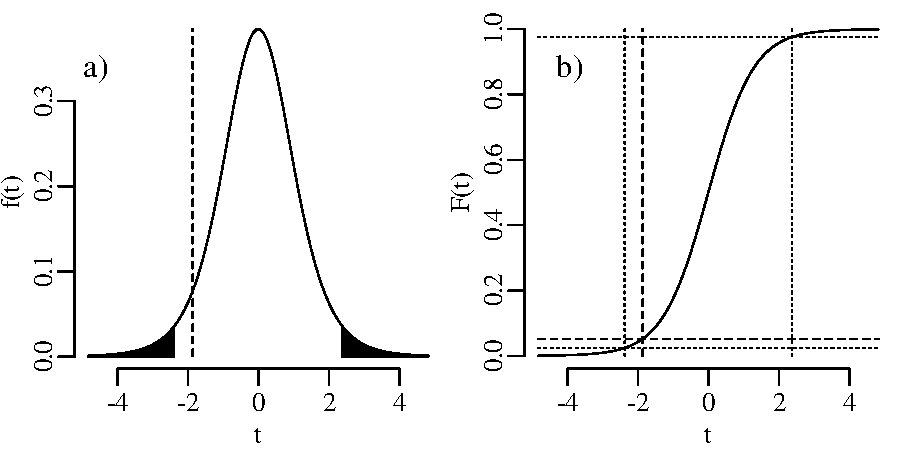
\includegraphics[width=\textwidth]{../figures/2samplettest.pdf}\medskip
\end{minipage}
\begin{minipage}[t][][t]{.4\textwidth}
  \captionof{figure}{a) PDF and b) CDF of a t-distribution with 7
    degrees of freedom. The two-sided rejection region (for
    $\alpha=0.05$) is marked in black. The vertical dashed line marks
    the observed value of $t=-1.857$ and plots outside the rejection
    region. Therefore the test does not allow us to conclude that
    $\mu_1\neq\mu_2$. }
  \label{fig:2samplettest}
\end{minipage}

\section{Confidence intervals}
\label{eq:tconf}

Section~\ref{sec:t} introduced a powerful way to test whether the mean
of a sample was equal to a particular value, or to the mean of another
sample. However, Section~\ref{sec:pitfalls} showed that formalised
tests such as the t-test have limited practical value. Provided that
the sample is large enough, its mean will nearly always be
`significantly' different than that of another sample. Suppose that we
were to average the densities of not five but five millions coins,
then it would be extremely unlikely for the mean to be exactly 19.30
g/cm\textsuperscript{3}. With a sample size of five million the power
of the t-test would be such that even trace amounts of a lighter
contaminant would have a detectable effect on the density.\medskip

Instead of asking ourselves whether the coins have the same density as
gold, it is more useful to know what the mean density actually is, and
to construct a confidence interval for it. We could then use this
information to learn something about the composition of the gold
coins. To construct a confidence interval for the mean, we follow a
similar procedure as laid out in Sections~\ref{sec:binomCI} and
\ref{sec:poisCI}. Let us use the first set of coins as an example, and
recall that the one sample t-statistic is defined as
(Equation~\ref{eq:t1}):
\[
  t = \frac{\bar{x} - \mu}{s[x]/\sqrt{n}}
\]

By definition, the 95\% confidence interval is the collection of all
those values of $\mu$ for which
\[
t_{df,\alpha/2} \leq t \leq t_{df,1-\alpha/2}
\]

\noindent where $t_{df,\alpha/2}$ and $t_{df,1-\alpha/2}$ are the
$\alpha/2$ and $(1-\alpha/2)$ quantiles of a t-distribution with $df$
degrees of freedom, respectively.  Hence:
\[
t_{df,\alpha/2} \leq \frac{\bar{x} - \mu}{s[x]/\sqrt{n}} \leq t_{df,1-\alpha/2}
\]

Rearranging:
\[
\bar{x} - t_{df,\alpha/2}\frac{s[x]}{\sqrt{n}} \geq \mu \geq
\bar{x} - t_{df,1-\alpha/2}\frac{s[x]}{\sqrt{n}}
\]

Because the t-distribution is symmetric around zero, we can also write:
\[
t_{df,1-\alpha/2} = -t_{df,\alpha/2}
\]

Hence
\[
\bar{x} + t_{df,\alpha/2}\frac{s[x]}{\sqrt{n}} \leq \mu \leq
\bar{x} - t_{df,\alpha/2}\frac{s[x]}{\sqrt{n}}
\]

\noindent or
\begin{equation}
  \mu \in \left\{\bar{x} \pm t_{df,\alpha/2}\frac{s[x]}{\sqrt{n}}\right\}
  \label{eq:tci}
\end{equation}

For the gold coin example of Section~\ref{sec:t}, $\bar{x}=19.164$,
$s[x]=0.0948$, $df=4$ and $t_{4,0.025}=-2.776$. Hence the 95\%
confidence interval for $\mu$ is
$19.16\pm{0.12}$~g/cm\textsuperscript{3}. Note that this interval does
\emph{not} overlap with the density of pure gold
(19.30~g/cm\textsuperscript{3}), confirming again that the coins are
not made of pure gold. However, the upper limit of the 95\% confidence
interval is 19.28~g/cm\textsuperscript{3}, which is not far off the
19.30~g/cm\textsuperscript{3} value. Therefore it is possible that the
amount of light contaminant is minor.\medskip

With increasing sample size, the t-distribution converges towards the
normal distribution:

\noindent\begin{minipage}[t][][b]{.6\textwidth}
  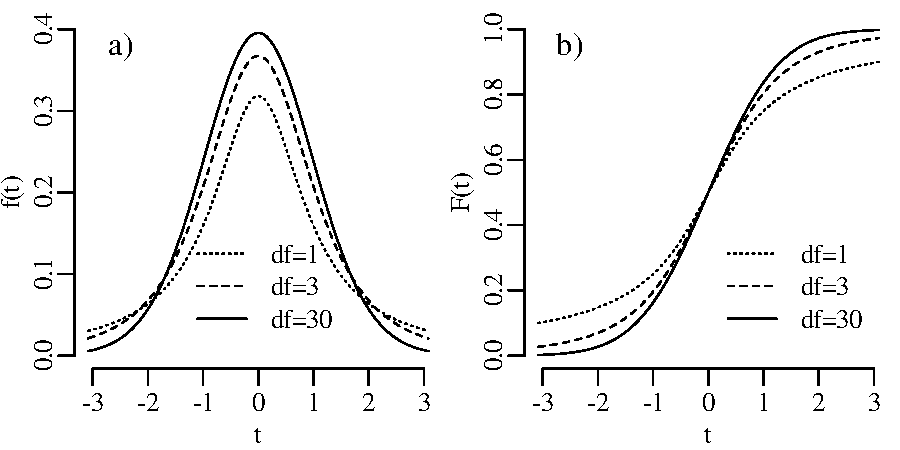
\includegraphics[width=\textwidth]{../figures/tdof.pdf}\medskip
\end{minipage}
\begin{minipage}[t][][t]{.4\textwidth}
  \captionof{figure}{a) PDFs and b) CDFs of the t-distribution for
    three different degrees of freedom ($df$). For small sample sizes
    (low $df$), the t-distribution has long tails towards low and high
    values. With increasing sample size, the tails become shorter and
    the t-distribution sharper. When $df>30$, the t-distribution is
    indistinguishable from a standard normal distribution with $\mu=0$
    and $\sigma=1$.}
  \label{fig:tdof}
\end{minipage}

Evaluating $t_{df,0.975}$ for different values of $df$:

\begin{center}
  \begin{tabular}{c|c@{\gap}c@{\gap}c@{\gap}c@{\gap}c@{\gap}c
      @{\gap}c@{\gap}c@{\gap}c@{\gap}c@{\gap}c@{\gap}c@{\gap}c}
    $df$ & 1 & 2 & 3 & 4 & 5 & 6 & 7 & 8 & 9 & 10 & 30 & 100 & 1000 \\
    $t_{df,0.975}$ &  12.710 & 4.303 & 3.182 & 2.776 & 2.571 &
    2.447 & 2.365 & 2.306 & 2.262 & 2.228 & 2.042 & 1.984 & \textbf{1.962}
  \end{tabular}
\end{center}

For large sample sizes, the 95\% percentile of the t-distribution is
the same as the 95\% percentile of the normal distribution ($=1.962$,
see Section~\ref{sec:normalproperties}). In this case
Equation~\ref{eq:tci} simplifies to approximately
\[
\mu \in \left\{ \bar{x} \pm 2 s[\bar{x}] \right\}
\]

\noindent where $s[\bar{x}]$ is the standard error of the mean
(Equation~\ref{eq:stderrmean}).

\noindent\begin{minipage}[t][][b]{.6\textwidth}
  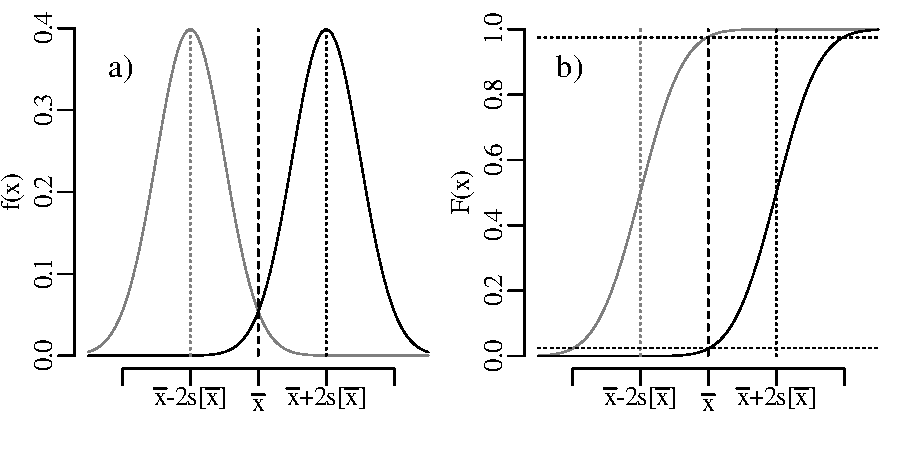
\includegraphics[width=\textwidth]{../figures/normconf.pdf}\medskip
\end{minipage}
\begin{minipage}[t][][t]{.4\textwidth}
  \captionof{figure}{The grey and black lines mark the PDFs (a) and
    CDFs (b) of two normal distributions whose means (vertical dotted
    lines) are offset by 2 standard errors from the sample average
    (vertical dashed line).  They mark a 95\% confidence interval for
    $\mu$. However this simple procedure only works if sample size is
    large enough for the Central Limit Theorem to apply.}
  \label{fig:normconf}
\end{minipage}

It is important to bear in mind that this procedure only works for
sufficiently large samples sizes. For samples sizes of $n<30$, the
`2-sigma' interval must be replaced with a `studentised' confidence
interval (i.e., Equation~\ref{eq:tci}).

\section{The $\chi^2$-test}
\label{sec:chi2}

Comparing the means of two datasets is one way to assess their
(dis)similarity. But as we have seen in Chapter~\ref{ch:plotting} and
Figure~\ref{fig:anscombe}, summary statistics like the mean do not
always capture the data adequately. The $\chi^2$ (chi-square) test is
an alternative approach, which uses a histogram to compare the
\emph{shape} of a sample distribution with a theoretical distribution,
or with another sample distribution.\medskip

To illustrate this method, let us go back to example~1 of
Chapter~\ref{ch:poisson}. Figure~\ref{fig:declusteredquakesperyear}
tallied the number of magnitude $\geq{5.0}$ earthquakes per year from
1917 to 2016.  This histogram represents 100 years, with values
ranging from 1 to 12 events per year. Based on the similarity of the
mean (5.43) and the variance (6.25), Chapter~\ref{ch:poisson}
proceeded under the assumption that the data followed a Poisson
distribution.  The $\chi^2$-test allows us to test this assumption
more rigorously.\medskip

We begin by counting the number of events in each bin of
Figure~\ref{fig:declusteredquakesperyear}:

\begin{center}
  \begin{tabular}{r|c@{\gap}c@{\gap}c@{\gap}c@{\gap}c@{\gap}
      c@{\gap}c@{\gap}c@{\gap}c@{\gap}c@{\gap}c@{\gap}c@{\gap}c}
    earthquakes/year &
    0 & 1 & 2 & 3 & 4 & 5 & 6 & 7 & 8 & 9 & 10 & 11 & 12 \\
    number of years &
    0 & 3 & 8 & 13 & 17 & 13 & 14 & 13 & 5 & 8 & 3 & 1 & 2 
  \end{tabular}
\end{center}

Next, we calculate the \textit{expected} number of events per bin
using the probability mass function of the Poisson distribution with
$\lambda=5.43$ (Equation~\ref{eq:poispmf}):

\begin{center}
  \begin{tabular}{r|c@{\gap}c@{\gap}c@{\gap}c@{\gap}c@{\gap}
      c@{\gap}c@{\gap}c@{\gap}c@{\gap}c@{\gap}c@{\gap}c@{\gap}c}
    earthquakes/year ($k$) &
    0 & 1 & 2 & 3 & 4 & 5 & 6 & 7 & 8 & 9 & 10 & 11 & 12 \\
    $N\times{P}(k|\lambda=5.43)$ &
    0.438 & 2.38 & 6.46 & 11.7 & 15.9 & 17.2 & 15.6 & 12.1 &
    8.22 & 4.96 & 2.69 & 1.33 & 0.601
  \end{tabular}
\end{center}

\noindent where $N=100$ years. In order for the $\chi^2$-test to work,
the bins should contain at least 5 items. We can fulfil these
requirements by \emph{pooling} the smallest bins.

\begin{center}
  \begin{tabular}{r|c@{\gap}c@{\gap}c@{\gap}
      c@{\gap}c@{\gap}c@{\gap}c@{\gap}c}
    earthquakes/year &
    $\leq{2}$ & 3 & 4 & 5 & 6 & 7 & 8 & $\geq{9}$ \\
    observed counts &
    11 & 13 & 17 & 13 & 14 & 13 & 5 & 14 \\
    predicted counts & 9.28 & 11.7 &
    15.9 & 17.2 & 15.6 & 12.1 & 8.22 & 9.98
  \end{tabular}
\end{center}

We can then compute the $\chi^2$-statistic:
\begin{equation}
  \chi^2 = \sum\limits_{i=1}^{n} \frac{(O_i-E_i)^2}{E_i}
  \label{eq:chi2}
\end{equation}

\noindent where $O_i$ stands for the observed and $E_i$ for the
expected number of counts in the $i$\textsuperscript{th} out of $n=8$
bins.\medskip

Finally we compare the value of $\chi^2$ with a chi-square
distribution with $n-2$ degrees of freedom, where one degree of
freedom has been removed because we forced
$\sum_{i=1}^nE_i=\sum_{i=1}^nO_i$, and another degree of freedom was
subtracted because we used the data to estimate $\lambda$ when
predicting the expected counts.\medskip

Applying the $\chi^2$-test to the earthquake data:

\begin{enumerate}
\item  Formulate two hypotheses:

  $H_0$ (\textbf{null hypothesis}):
  the earthquake data follow a Poisson distribution

  $H_{\!A}$ (\textbf{alternative hypothesis}):
  the earthquake data do not follow a Poisson distribution
  
\item Calculate the $\chi^2$-statistic using Equation~\ref{eq:chi2}:
  \begin{equation}
    \begin{split}
      \chi^2 = &
      \frac{(11-9.28)^2}{9.28} + \frac{(13-11.7)^2}{11.7} +
      \frac{(17-15.9)^2}{15.9} + \frac{(13-17.2)^2}{17.2} + \\
      & \frac{(14-15.6)^2}{15.6} + \frac{(13-12.1)^2}{12.1} +
      \frac{(5-8.22)^2}{8.22} + \frac{(14-9.98)^2}{9.98} = 4.70
    \end{split}
  \end{equation}

\item Under $H_0$, Equation~\ref{eq:chi2} follows a
  $\chi^2$-distribution 6 degrees of freedom. Tabulating some key
  quantiles for this distribution:

  \begin{center}
    \begin{tabular}{c|c@{\gap}c@{\gap}c@{\gap}c@{\gap}
        c@{\gap}c@{\gap}c@{\gap}c@{\gap}c@{\gap}c@{\gap}c@{\gap}c}
      $\chi^2$ & 0.872 & 1.24 & 1.64 & 2.20 & 3.45 & \textit{4.70} &
      5.35 & 7.84 & 10.6 & 12.6 & 14.4 & 16.8 \\ \hline
      $P(X\leq{\chi^2})$ & 0.01 & 0.025 & 0.05 & 0.1 & 0.25 &
      \textit{0.417} & 0.5 & 0.75 & 0.9 & 0.95 & 0.975 & 0.99 \\
      $P(X\geq{\chi^2})$ & 0.99 & 0.975 & 0.95 & 0.9 & 0.75 &
      \textit{0.583} & 0.5 & 0.25 & 0.1 & 0.05 & 0.025 & 0.01
    \end{tabular}
  \end{center}

  \noindent where the observed value is marked in italics.
  
\item We will use an $\alpha = 0.05$ confidence level.

\item We are only interested in the upper tail of the null
  distribution, because this indicates sample distributions that are
  very dissimilar from the theoretical distribution. The lower tail of
  the distribution groups samples that are very similar to the
  predicted distribution (see Section~\ref{sec:cherrypicking} for
  further discussion). Marking the rejection region in bold:
  
  \begin{center}
    \begin{tabular}{c|c@{\gap}c@{\gap}c@{\gap}c@{\gap}
        c@{\gap}c@{\gap}c@{\gap}c@{\gap}c@{\gap}c@{\gap}c@{\gap}c}
      $\chi^2$ & 0.872 & 1.24 & 1.64 & 2.20 & 3.45 & \textit{4.70} &
      5.35 & 7.84 & 10.6 & \textbf{12.6} &
      \textbf{14.4} & \textbf{16.8} \\ \hline
      $P(X\geq{\chi^2})$ & 0.99 & 0.975 & 0.95 & 0.9 & 0.75 &
      \textit{0.743} & 0.5 & 0.25 & 0.1 & \textbf{0.05} &
      \textbf{0.025} & \textbf{0.01}
    \end{tabular}
  \end{center}

  The one-sided rejection region consists of all $\chi^2>{12.6}$. 

\item Because the observed value of $\chi^2=4.70$ falls outside the
  rejection region, we cannot reject the null hypothesis.

\end{enumerate}

\noindent\begin{minipage}[t][][b]{.6\textwidth}
  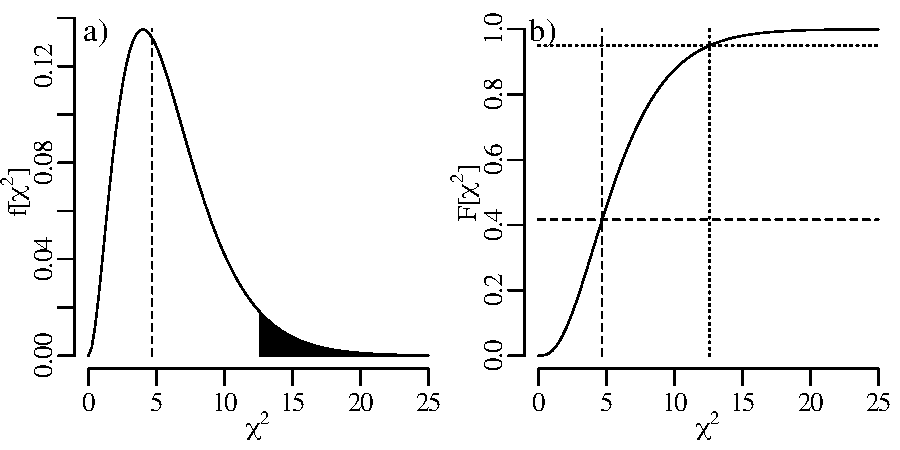
\includegraphics[width=\textwidth]{../figures/chi2.pdf}\medskip
\end{minipage}
\begin{minipage}[t][][t]{.4\textwidth}
  \captionof{figure}{a) PDF and b) CDF of the $\chi^2$-distribution
    with 6 degrees of freedom. The rejection region is marked in
    black.  The observed value for the earthquake data ($\chi^2=4.70$)
    is shown as a vertical dashed line.  It plots outside the
    rejection region, indicating that the histogram of the data falls
    within the expected range of the hypothesised (Poisson)
    distribution.  }
  \label{fig:chi2}
\end{minipage}

\section{Comparing two or more samples}
\label{sec:contingency}

Recall that the t-test of Section~\ref{sec:t} could either be used to
compare the mean of a single sample with a particular value, or to
compare the means of two samples. In a similar vein, the $\chi^2$-test
can be used to compare either one sample to a theoretical
distribution, or to compare two samples with each other. For example,
let us compare two sets of petrographic observations:

\begin{center}
  \begin{tabular}{r|cccc}
~ & quartz & plagioclase & alkali feldspar & lithics \\ \hline
sample A & 10 & 5 & 6 & 20 \\
sample B & 25 & 12 & 10 & 35
  \end{tabular}
  \captionof{table}{Manual point counting data for two samples of
    sand.}
  \label{tab:observedclasts}
\end{center}

This is a ${2}\times{4}$ \textbf{contingency table}. Note that the two
samples contain a different number of clasts.

\begin{center}
  \begin{tabular}{r|cccc|c}
lithology & quartz & plagioclase & alkali feldspar & lithics & row sum \\ \hline
sample A & 10 & 5 & 6 & 20 & 41\\
sample B & 25 & 12 & 10 & 35 & 82 \\ \hline
column sum & 35 & 17 & 16 & 55 & 123
  \end{tabular}
\end{center}

If the two samples have the same underlying composition, then the
expected counts of each cell in the contingency table should be:
\[
\mbox{expected counts of bin }(i,j) =
\frac{(\mbox{sum of row }i)\times(\mbox{sum of column }j)}
     {(\mbox{sum of all the cells})}
\]

For example, the expected number of quartz grains in sample~A would be
\[
\frac{41\times35}{123}=11.7
\]

Applying this formula to the whole table, the expected counts are

\begin{center}
  \begin{tabular}{r|cccc}
lithology & quartz & plagioclase & alkali feldspar & lithics \\ \hline
sample A & 11.7 & 5.67 & 5.33 & 18.3 \\
sample B & 23.3 & 11.30 & 10.70 & 36.7
  \end{tabular}
  \captionof{table}{Expected grain counts for two sedimentary samples.}
  \label{tab:expectedclasts}
\end{center}

All the cells in this table exceed 5. Therefore, the observed
(table~\ref{tab:observedclasts}) and expected
(table~\ref{tab:expectedclasts}) counts can be plugged into
Equation~\ref{eq:chi2} to calculate a $\chi^2$-value. The null
distribution of this statistic is $\chi^2$ with $(n_r-1)\times(n_c-1)$
degrees of freedom, where $n_r$ is the number of rows and $n_c$ is the
number of columns.  The $\chi^2$-test then proceeds in the same way as
the one-sample case of Section~\ref{sec:chi2}:

\begin{enumerate}
\item  Formulate two hypotheses:

  $H_0$ (\textbf{null hypothesis}): samples A and B have the same composition

  $H_{\!A}$ (\textbf{alternative hypothesis}):
  samples A and B do not have the same composition
  
\item Calculate the $\chi^2$-statistic with Equation~\ref{eq:chi2},
  using table~\ref{tab:observedclasts} for the observed and
  table~\ref{tab:expectedclasts} for the predicted values:
  \begin{equation}
    \begin{split}
      \chi^2 = &
      \frac{(10-11.7)^2}{11.7} + \frac{(5-5.67)^2}{5.67} +
      \frac{(6-5.33)^2}{5.33} + \frac{(20-18.3)^2}{18.3} + \\
      & \frac{(25-23.3)^2}{23.3} + \frac{(12-11.30)^2}{11.30} +
      \frac{(10-10.70)^2}{10.70} + \frac{(35-36.7)^2}{36.7} = 0.86
    \end{split}
  \end{equation}

\item Under $H_0$, Equation~\ref{eq:chi2} follows a
  $\chi^2$-distribution with $(2-1)\times(4-1)=3$ degrees of
  freedom. Tabulating some key quantiles for this distribution:

  \begin{center}
    \begin{tabular}{c|c@{\gap}c@{\gap}c@{\gap}c@{\gap}
        c@{\gap}c@{\gap}c@{\gap}c@{\gap}c@{\gap}c@{\gap}c@{\gap}c}
      $\chi^2$ & 0.115 & 0.216 & 0.352 & 0.584 & \textit{0.86} &
      1.21 & 2.37 & 4.11 & 6.25 & 7.81 & 9.35 & 11.3 \\ \hline
      $P(X\leq{\chi^2})$ & 0.01 & 0.025 & 0.05 & 0.1 & \textit{0.157} &
      0.25 & 0.5 & 0.75 & 0.9 & 0.95 & 0.975 & 0.99 \\
      $P(X\geq{\chi^2})$ & 0.99 & 0.975 & 0.95 & 0.9 & \textit{0.843} & 
      0.75 & 0.5 & 0.25 & 0.1 & 0.05 & 0.025 & 0.01
    \end{tabular}
  \end{center}

  \noindent where the observed value is marked in italics.
  
\item The confidence level $\alpha = 0.05$.

\item Marking the rejection region in bold:
  
  \begin{center}
    \begin{tabular}{c|c@{\gap}c@{\gap}c@{\gap}c@{\gap}
        c@{\gap}c@{\gap}c@{\gap}c@{\gap}c@{\gap}c@{\gap}c@{\gap}c}
      $\chi^2$ & 0.115 & 0.216 & 0.352 & 0.584 & \textit{0.86} &
      1.21 & 2.37 & 4.11 & 6.25 & \textbf{7.81} &
      \textbf{9.35} & \textbf{11.3} \\ \hline
      $P(X\geq{\chi^2})$ & 0.99 & 0.975 & 0.95 & 0.9 & \textit{0.843} & 
      0.75 & 0.5 & 0.25 & 0.1 & \textbf{0.05} &
      \textbf{0.025} & \textbf{0.01}
    \end{tabular}
  \end{center}

  The one-sided rejection region consists of all $\chi^2>{7.81}$.

\item Because the observed value of $\chi^2=0.86$ falls outside this
  region, we cannot reject the null hypothesis.

\end{enumerate}

\noindent\begin{minipage}[t][][b]{.6\textwidth}
  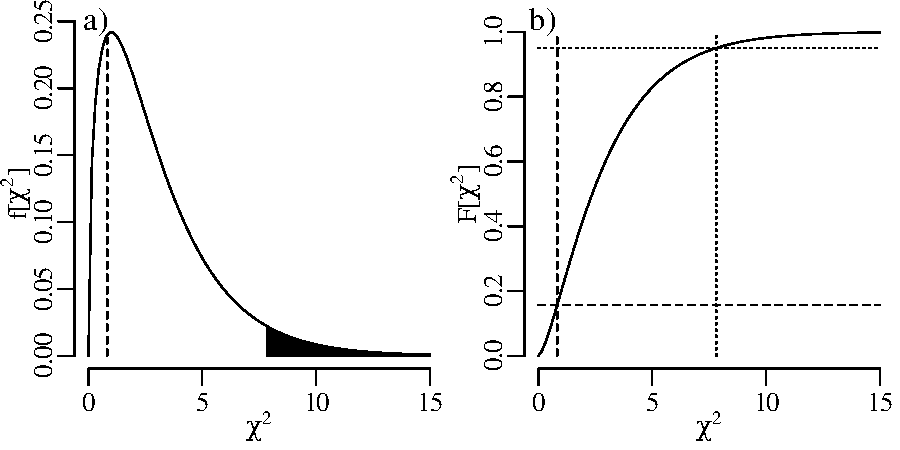
\includegraphics[width=\textwidth]{../figures/chi22.pdf}\medskip
\end{minipage}
\begin{minipage}[t][][t]{.4\textwidth}
  \captionof{figure}{a) PDF and b) CDF of the $\chi^2$-distribution
    with 3 degrees of freedom. The rejection region is marked in
    black.  The observed value ($\chi^2=0.86$) is shown as a vertical
    dashed line.  It plots outside the rejection region, indicating
    that the histogram of the data falls within the expected range of
    the hypothesised (Poisson) distribution.  }
  \label{fig:chi22}
\end{minipage}

\section{Cherry picking (Type-I errors revisited)}
\label{sec:cherrypicking}

The $\chi^2$-distribution only covers positive numbers, from 0 to
$\infty$. Low $\chi^2$-values indicate a good fit of the data to the
proposed distribution, and high $\chi^2$-values indicate a bad fit.
This is why the $\chi^2$-tests of Section~\ref{sec:chi2} were
one-tailed tests: we want to identify the bad fits in order to reject
the null hypothesis. However it would be wrong to completely ignore
the good fits.\medskip

Section~\ref{sec:pitfalls} made the case that, in general, the desired
outcome of a statistical test is the rejection of the null hypothesis.
However, in the context of distributional tests, our life is often
easier if the null hypothesis is \emph{not} rejected. For example, if
the data pass a $\chi^2$-test for a Poisson distribution, then this
allows us to model the data with a single number ($\lambda$). If the
data fail the $\chi^2$-test, then we may have to abandon the
simplicity of the Poisson distribution and use a more realistic but
complex alternative.\medskip

The desire to see the data pass a hypothesis test leads some
scientists to \textbf{cherry pick} data. This means that they
selectively remove perceived `outliers' from the data until the
remaining values pass the null hypothesis. It is important to remember
that, even if the null hypothesis is true, we should still expect 5\%
(if $\alpha=0.05$) of all samples fail the null hypothesis. That is,
there is always a 5\% chance of committing a Type-I error
(Section~\ref{sec:typeI&II}).\medskip

If all samples in a study have p-values exceeding 0.05, then this
should raise suspicion. For example, comparing a Poisson null
distribution (a) with three samples (b--d):

\noindent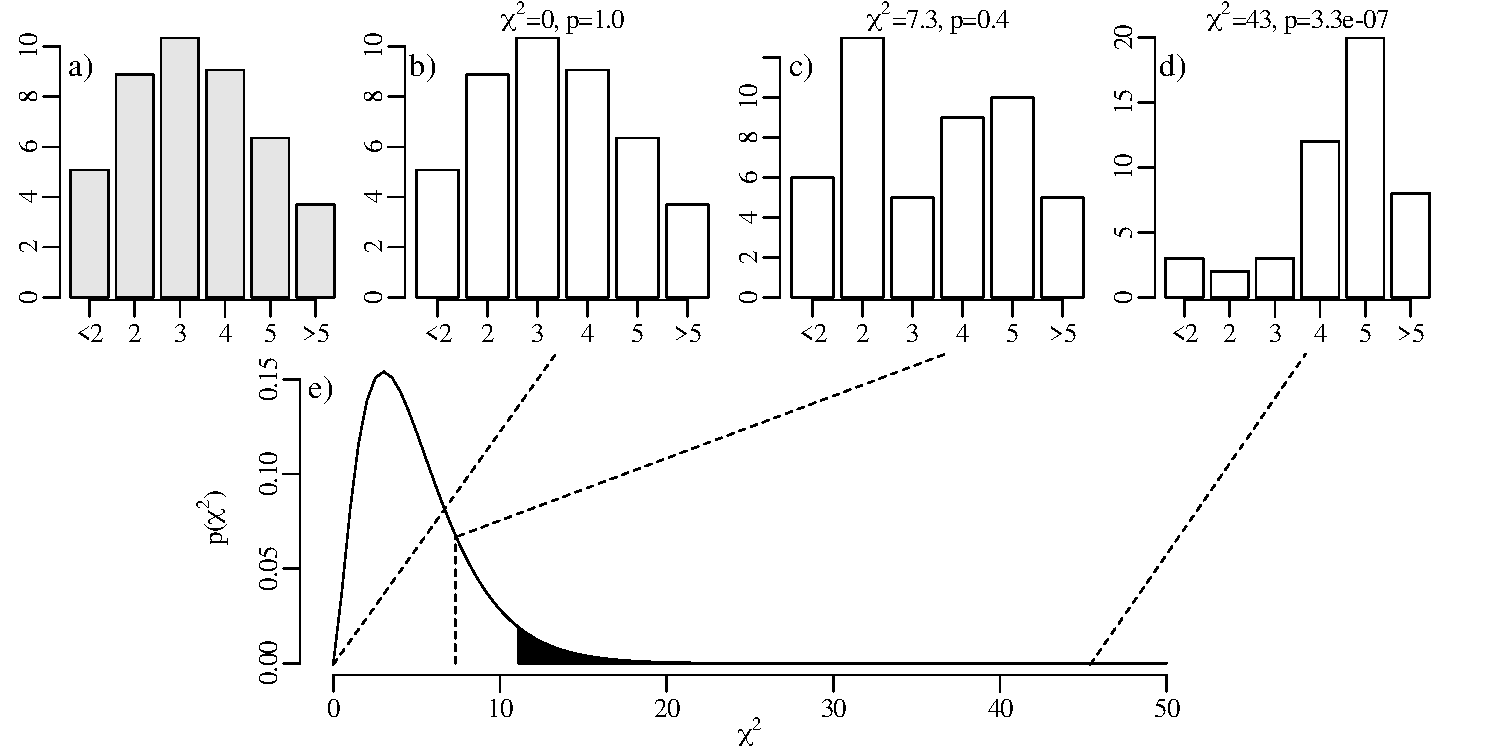
\includegraphics[width=\textwidth]{../figures/cherrypicking.pdf}\medskip
\begingroup
\captionof{figure}{a) predicted frequency distribution for the zircon
  count data of example~2 in Chapter~\ref{ch:poisson}, following a Poisson
  distribution with $\lambda=3.50$ and $n=48$; b) -- d) three sample
  distributions with the $\chi^2$ statistic and p-values for
  comparison with distribution a; e) $\chi^2$-distribution with 5
  degrees of freedom.  The $\chi^2$-test would flag sample d as being
  `significantly different' from the predicted histogram a. Sample c
  also looks somewhat different from the predicted distribution a, but
  this difference falls within the expected range of random sampling
  variability of the Poisson distribution. Sample b is identical to
  the prediction a. This should raise suspicion. It is extremely
  unlikely for a sample to fit the prediction so well.\medskip}
  \label{fig:cherrypicking}
\endgroup

The first sample is identical to the predicted distribution
($\chi^2$-statistic = 0.0, p-value = 1.0).  Such an extraordinarily
`good' result would be extremely unlikely to happen by chance.

\section{Effect size (Type-II errors revisited)}
\label{sec:effectsize}

Let us carry out a similar experiment to
Section~\ref{sec:contingency}, but instead of counting a few
sedimentary clasts by hand, we task a machine to classify $\sim$10,000
grains of sand by image recognition:

\begin{center}
  \begin{tabular}{r|cccc}
    lithology & quartz & plagioclase & alkali feldspar & lithics  \\ \hline
    sample A & 29544 & 14424 & 13706 & 47864 \\
    sample B & 29454 & 14788 & 13948 & 47311
  \end{tabular}
  \captionof{table}{Automated point counting data for two samples of sand.}
  \label{tab:observedsand}
\end{center}

At first glance, the two samples look very similar in composition. But
let's carry out a two-sample $\chi^2$-test to be sure.

\begin{enumerate}
\item  Formulate two hypotheses:

  $H_0$ (\textbf{null hypothesis}):
  samples A and B have identical compositions

  $H_{\!A}$ (\textbf{alternative hypothesis}):
  samples A and B have different compositions
  
\item The expected number of counts for each cell of the contingency
  table is obtained using the procedure outlined in
  Section~\ref{sec:contingency}. Calculate the row and column sums:

  \begin{center}
    \begin{tabular}{r|cccc|c}
      lithology & quartz & plagioclase & alkali feldspar &
      lithics & row sum \\ \hline
      sample A & 29544 & 14424 & 13706 & 47864 & 105538 \\
      sample B & 29454 & 14788 & 13948 & 47311 & 105501 \\ \hline
      column sum & 58998 & 29212 & 27654 & 95175 & 211039
    \end{tabular}
  \end{center}

  \noindent and combine them to produce the following predicted
  counts:

  \begin{center}
    \begin{tabular}{r|cccc}
      lithology & quartz & plagioclase & alkali feldspar & lithics  \\ \hline
      sample A & 29504 & 14609 & 13829 & 47596 \\
      sample B & 29494 & 14603 & 13825 & 47579 \\
    \end{tabular}
    \captionof{table}{Predicted point counts.}
    \label{tab:predictedsand}
  \end{center}

  Plugging tables~\ref{tab:observedsand} and \ref{tab:predictedsand}
  into Equation~\ref{eq:chi2} yields
  \[
  \chi^2 = 10.0
  \]

\item Under $H_0$, the test statistic follows a
  $\chi^2$-distribution 3 degrees of freedom. Tabulating some key
  quantiles for this distribution:

  \begin{center}
    \begin{tabular}{c|c@{\gap}c@{\gap}c@{\gap}c@{\gap}
        c@{\gap}c@{\gap}c@{\gap}c@{\gap}c@{\gap}c@{\gap}c@{\gap}c}
      $\chi^2$ & 0.115 & 0.216 & 0.352 & 0.584 & 1.21 & 2.37 &
      4.11 & 6.25 & 7.81 & 9.35 & \textit{10.0} & 11.3 \\ \hline
      $P(X\leq{\chi^2})$ & 0.01 & 0.025 & 0.05 & 0.1 & 0.25 &
      0.5 & 0.75 & 0.9 & 0.95 & 0.975 & \textit{0.9814} & 0.99 \\
      $P(X\geq{\chi^2})$ & 0.99 & 0.975 & 0.95 & 0.9 & 0.75 & 0.5 &
      0.25 & 0.1 & 0.05 & 0.025 & \textit{0.0186} & 0.010
    \end{tabular}
  \end{center}

  \noindent where the observed value is marked in italics.
  
\item The confidence level $\alpha = 0.05$.

\item Marking the rejection region in bold:
  
  \begin{center}
    \begin{tabular}{c|c@{\gap}c@{\gap}c@{\gap}c@{\gap}
        c@{\gap}c@{\gap}c@{\gap}c@{\gap}c@{\gap}c@{\gap}c@{\gap}c}
      $\chi^2$ & 0.115 & 0.216 & 0.352 & 0.584 & 1.21 & 2.37 &
      4.11 & 6.25 & \textbf{7.81} & \textbf{9.35} &
      \textbf{\textit{10.0}} & \textbf{11.3} \\ \hline
      $P(X\geq{\chi^2})$ & 0.99 & 0.975 & 0.95 & 0.9 & 0.75 & 0.5 &
      0.25 & 0.1 & \textbf{0.05} & \textbf{0.025} &
      \textbf{\textit{0.0186}} & \textbf{0.010}
    \end{tabular}
  \end{center}

  The one-sided rejection region consists of all $\chi^2>{7.81}$.

\item The observed value of $\chi^2=10.0$ falls inside this region,
  and so we reject $H_0$.

\end{enumerate}

So despite the close similarity of the point counts for samples A and
B in table~\ref{tab:observedsand}, the $\chi^2$-test convincingly
rejects the null hypothesis that they were drawn from the same
population. To understand what is going on, we need to go back to
Section~\ref{sec:pitfalls}. This section explained that the power of a
statistical test to evaluate a null hypothesis monotonically increases
with sample size.\medskip

With more than 100,000 counts per sample, it is not surprising that
the $\chi^2$-test is able to detect even the tiniest difference
between samples A and B.  In comparison, the two samples of
Section~\ref{sec:contingency} only contain 41 and 82 samples,
respectively. Consequently, it is more difficult to detect a small
difference in composition between them.\medskip

The power of a statistical test depends on two things:

\begin{enumerate}
  \item Sample size: the larger the sample size, the easier it is to
    reject a false null hypothesis.
  \item The \emph{degree to which the null hypothesis is false}: the
    greater the difference between the underlying populations, the
    easier it is to recognise this difference in the samples.
\end{enumerate}

The second aspect can be quantified as the \textbf{effect size}. In
the case of the $\chi^2$-distribution, the effect size is defined as:
\begin{equation}
  w = \sqrt{\sum\limits_{i=1}^{n}\frac{\left(o_i-e_i\right)^2}{e_i}}
  \label{eq:effectsize}
\end{equation}

\noindent where $o_i=O_i/N$ and $e_i=E_i/N$ with
$N=\sum_{i}^{n}O_i=\sum_{i}^{n}E_i$.  Effect sizes can be small,
medium or large:

\begin{center}
  \begin{tabular}{c|ccc}
    effect size & small & medium & large \\ \hline
    $w$ & 0.1 & 0.3 & 0.5
  \end{tabular}
\end{center}

For the framework mineral counts,

\begin{center}
  \begin{tabular}{rr|cccc}
    & lithology & quartz & plagioclase & alkali feldspar & lithics  \\
    \cline{2-6}
    $o$ = & sample A & 0.1400 & 0.06835 & 0.06495 & 0.2268 \\
    & sample B & 0.1396 & 0.07007 & 0.06609 & 0.2242
  \end{tabular}
\end{center}

\noindent and

\begin{center}
  \begin{tabular}{rr|cccc}
    & lithology & quartz & plagioclase & alkali feldspar & lithics  \\
    \cline{2-6}
    $e$ = & sample A & 0.1398 & 0.06922 & 0.06553 & 0.2255 \\
    & sample B & 0.1398 & 0.06920 & 0.06551 & 0.2255
  \end{tabular}
\end{center}

Plugging these values into Equation~\ref{eq:effectsize} yields an
effect size of $w=0.00688$, which is very small indeed. With a smaller
sample size, the difference between $A$ and $B$ would have gone
unnoticed.  The only reason why the $\chi^2$-test failed is the huge
size of the two samples. The tiny effect size indicates that, although
the difference between samples $A$ and $B$ may be statistically
significant, it is not \textit{geologically significant}.

\section{Non-parametric tests}
\label{sec:nonparametric}

The t-test and $\chi^2$-test make specific parametric assumptions
about the data:

\begin{itemize}
  \item The t-test assumes that the population mean follows a normal
    distribution. This assumption may not be correct for small samples
    from multimodal distributions. For example, when averaging $n=2$
    or $n=3$ values from the bimodal geyser data
    (Figures~\ref{fig:CLTfaithful2} and \ref{fig:CLTfaithful3}), the
    assumption of normality is clearly incorrect.
  \item The $\chi^2$-test requires binning the data into a
    histogram. This makes it well suited for discrete distributions
    such as the binomial and Poisson distribution. However it is less
    well adapted to continuous distributions such as the normal
    distribution. Furthermore, each bin in the histogram requires a
    sufficient number of counts for the $\chi^2$-assumption to be
    valid. This requirement may not be fulfilled for small samples.
\end{itemize}

These limitations can be avoided with \textbf{non-parametric tests},
which offer greater flexibility than parametric tests whilst
increasing robustness to outliers.\medskip

The \textbf{Wilcoxon test} (which is also known as the Mann-Whitney
test) is a non-parametric alternative to the t-test. Consider two sets
of numbers, representing two different samples:

\begin{center}
\begin{tabular}{r|ccccc}
 sample & 1 & 2 & 3 & 4 & 5 \\ \hline
 $A$ & $A_1$ & $A_2$ & $A_3$ & $A_4$ & $A_5$ \\
 $B$ & $B_1$ & $B_2$ & $B_3$ & $B_4$ 
\end{tabular}
\label{tab:mannwhitneygeneric}
\end{center}

\noindent To calculate the test statistic, merge the two samples and
rank them.  For example, suppose that $A_4 < A_1 < B_3 < A_2  < A_5 <
B_1 < A_3 < B_4 < B_2$. Then

\begin{center}
\begin{tabular}{c|ccccccccc}
  rank & 1 & 2 & 3 & 4 & 5 & 6 & 7 & 8 & 9 \\ \hline
  value & $A_4$ & $A_1$ & $B_3$ & $A_2$ & $A_5$ & $B_1$ & $A_3$ & $B_4$ & $B_2$
\end{tabular}
\end{center}

If the two samples follow the same distribution, then we would expect
the values to be randomly shuffled and evenly distributed on either
side of the median. However if the two samples follow different
distributions, then their values will be unevenly distributed.  The
test statistic is given by the sum of the ranks of the smallest
sample. In our case, sample $A$ contains 5 and sample $B$ 4 items.
Thus we calculate sum of the ranks of sample $B$:
\[
W = 3 + 6 + 8 + 9 = 26
\]

For sample sizes of $n_A=5$ and $n_B=4$, $W$ takes on values between
$\sum_{i=1}^{4}i=10$ and $\sum_{i=6}^{9}i=30$. The closer the
$W$-value is to these extremes, the less likely it is that samples $A$
and $B$ were drawn from the same distribution. The hypothesis test is
carried out by comparing $W$ with a lookup table. To understand how
this lookup table is constructed, let us consider the smallest
possible outcome for $W$, which is $W=10$. This outcome corresponds to
the following arrangements:

\begin{center}
  \begin{tabular}{r|ccccccccc}
    arrangement 1: & $B_1$ & $B_2$ & $B_3$ & $B_4$ & $A_1$ &
    $A_2$ & $A_3$ & $A_4$ & $A_5$ \\
    arrangement 2: & $B_2$ & $B_1$ & $B_3$ & $B_4$ & $A_1$ &
    $A_2$ & $A_3$ & $A_4$ & $A_5$ \\
    arrangement 2: & $B_1$ & $B_2$ & $B_3$ & $B_4$ & $A_2$ &
    $A_1$ & $A_3$ & $A_4$ & $A_5$ \\
    etc. & & & & & & & & & 
  \end{tabular}
\end{center}

The total number of arrangements that result in $W=10$ is $4!5!$ (2880
possibilities). To compute the probability of $W=10$ under the null
hypothesis, we must divide this value by the total number of
permutations of the 9 values, which is $9!$ (see
Section~\ref{sec:permutations}). Therefore:
\[
P(W=10|n_A=5,n_B=4) = \frac{4!5!}{9!} = 0.00794
\]

The probability of other outcomes is computed in a similar fashion.\medskip

Let us illustrate the Wilcoxon rank-sum test with the two-sample
example of table~\ref{tab:2setcoins}:

\begin{center}
\begin{tabular}{c|ccccc}
  coin \# & 1 & 2 & 3 & 4 & 5 \\ \hline
  density (1\textsuperscript{st} collection) &
  19.09 & 19.17 & 19.31 & 19.07 & 19.18 \\
  density (2\textsuperscript{nd} collection) &
  \textbf{19.30} & \textbf{19.33} & \textbf{19.15} & \textbf{19.32}
\end{tabular}
\captionof{table}{The same data as table~\ref{tab:2setcoins} but with
  the second sample marked in bold for future use.}
\label{tab:mannwhitneycoins}
\end{center}

\begin{enumerate}
\item  Formulate two hypotheses:

  \noindent\begin{minipage}{.4\textwidth}
    $H_0$ (\textbf{null hypothesis})
    
    \vspace{1em}
    
    $H_{\!A}$ (\textbf{alternative hypothesis}):
  \end{minipage}
  \begin{minipage}{.2\textwidth}
  \end{minipage}
  \begin{minipage}{.4\textwidth}
    median(sample 1) = median(sample 2)
    
    \vspace{1em}
    
    median(sample 1) $\neq$ median(sample 2)
  \end{minipage}
  
\item To calculate the test statistic, merge the two samples and rank
  them:

  \begin{center}
    \begin{tabular}{c|ccccccccc}
      rank & 1 & 2 & \textbf{3} & 4 & 5 & \textbf{6} & 7 &
      \textbf{8} & \textbf{9} \\ \hline
      density & 19.07 & 19.09 & \textbf{19.15} & 19.17 & 19.18 &
      \textbf{19.30} & 19.31 & \textbf{19.32} & \textbf{19.33}
    \end{tabular}
  \end{center}

  \noindent where tied values have been given an average rank. The
  test statistic is then simply the sum of the ranks for the smallest
  sample:
  \begin{equation*}
    \begin{split}
      W = & 3 + 6 + 8 + 9 = 26
    \end{split}
  \end{equation*}

  \noindent which (intentionally) is the same value as the earlier
  generic example.

\item Under $H_0$, the test statistic follows a Wilcoxon rank-sum
  distribution for $n_1=5$ and $n_2=4$. Tabulating some key values for
  this distribution:

  \begin{center}
    \begin{tabular}{c|c@{\gap}c@{\gap}c@{\gap}c@{\gap}c@{\gap}c@{\gap}c@{\gap}c@{\gap}c@{\gap}c@{\gap}c@{\gap}c}
      $W$ & 10 & 11 & 12 & 13 & 19 & 20 & \textit{26} & 27 & 28 & 29 & 30 \\ \hline
      $P(w\leq{W})$ & 0.008 & 0.016 & 0.032 & 0.056 & 0.45 & 0.55 & \textit{0.944} & 0.97 & 0.98 & 0.99 & 1.0 \\
      $P(w\geq{W})$ & 1.0 & 0.99 & 0.98 & 0.97 & 0.63 & 0.55 & \textit{0.095} & 0.056 & 0.032 & 0.016 & 0.008
    \end{tabular}
  \end{center}

  \noindent where the observed value is marked in italics.
  
\item The confidence level $\alpha = 0.05$.

\item Marking the two-sided rejection region in bold:
  
  \begin{center}
    \begin{tabular}{c|c@{\gap}c@{\gap}c@{\gap}c@{\gap}c@{\gap}c@{\gap}c@{\gap}c@{\gap}c@{\gap}c@{\gap}c@{\gap}c}
      $W$ & \textbf{10} & \textbf{11} & 12 & 13 & 19 & 20 & \textit{26} & 27 & 28 & \textbf{29} & \textbf{30} \\ \hline
      $P(w\leq{W})$ & \textbf{0.008} & \textbf{0.016} & 0.032 & 0.056 & 0.45 & 0.55 & \textit{0.944} & 0.97 & 0.98 & 0.99 & 1.0 \\
      $P(w\geq{W})$ & 1.0 & 0.99 & 0.98 & 0.97 & 0.63 & 0.55 & \textit{0.095} & 0.056 & 0.032 & \textbf{0.016} & \textbf{0.008}
    \end{tabular}
  \end{center}

  The rejection region consists of $W=\{10,11,29,30\}$.

\item The observed value of $W (=26)$ falls outside the rejection
  region, and so we cannot reject $H_0$.

\end{enumerate}

\noindent\begin{minipage}[t][][b]{.6\textwidth}
  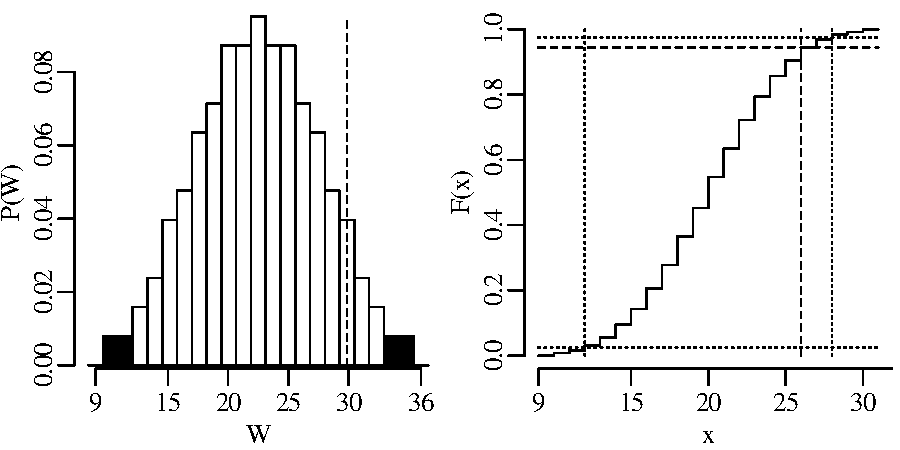
\includegraphics[width=\textwidth]{../figures/wilcox.pdf}\medskip
\end{minipage}
\begin{minipage}[t][][t]{.4\textwidth}
  \captionof{figure}{a) PMF and b) CDF of the Wilcoxon test statistic
    for comparison of two samples containing 5 and 4 items,
    respectively.  The two-sided rejection region is marked in black.
    The observed value ($W=26$) is shown as a vertical dashed line.
    It plots outside the rejection region, leaving open the
    possibility that the two samples might have come from the same
    distribution.}
  \label{fig:wilcox}
\end{minipage}

The \textbf{Kolmogorov-Smirnov test} is a non-parametric alternative
to the $\chi^2$-test that does not require binning. Given two sets of
numbers:
\[
x = \{x_1,x_2,\ldots,x_n\} \mbox{~and~} y = \{y_1,y_2,\ldots,y_m\}
\]

\noindent the Kolmogorov-Smirnov statistic is defined as the maximum
vertical distance between the ECDFs (Section~\ref{sec:ECDF}) of the
two samples:
\begin{equation}
  D = \underset{z}{\mbox{max}} |F_x(z) - F_y(z)|
  \label{eq:KS}
\end{equation}

\noindent where $F_x$ and $F_y$ are the ECDFs of $x$ and $y$,
respectively.  $D$ takes on values from 0 (two identical
distributions) and 1 (no overlap between the two distributions).\medskip

To illustrate the Kolmogorov-Smirnov method, consider two sand samples
from China: one sample from the Yellow River, and one sample from a
sand dune in the nearby Mu Us desert. We have separated the mineral
zircon from the sand and analysed the crystallisation age of $>100$
randomly selected zircon grains with the U--Pb method.  The frequency
distribution of the zircon dates serves as a characteristic
`fingerprint' that can be used to compare the different samples.

\noindent\begin{minipage}[t][][b]{.35\textwidth}
  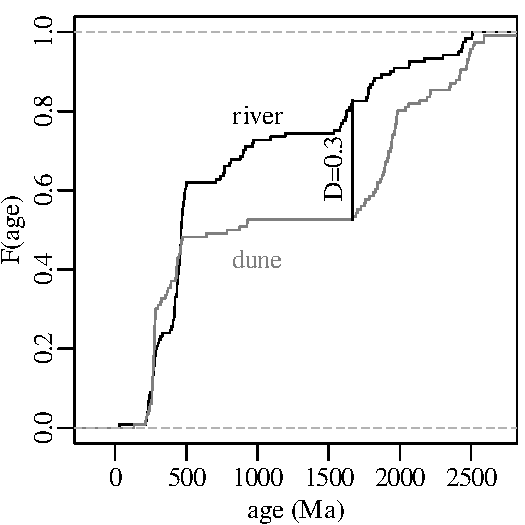
\includegraphics[width=\textwidth]{../figures/KS.pdf}\medskip
\end{minipage}
\begin{minipage}[t][][t]{.65\textwidth}
  \captionof{figure}{The two-sample Kolmogorov-Smirnov statistic is
    the maximum vertical distance between two ECDFs. This example
    compares the cumulative distributions of 121 detrital zircon U--Pb
    ages from the Yellow River with 116 detrital zircon U--Pb ages
    from a sand dune in the adjacent Mu Us desert. The KS-distance is
    0.3006.}
  \label{fig:KS}
\end{minipage}

The hypothesis test then proceeds as always:

\begin{enumerate}
\item  Formulate two hypotheses:

  $H_0$ (\textbf{null hypothesis}):
  samples 1 and 2 were drawn from the same distribution

  $H_{\!A}$ (\textbf{alternative hypothesis}):
  samples 1 and 2 were drawn from different distributions
  
\item The test statistic is $D=0.30$ (see Figure~\ref{fig:KS}).

\item Under $H_0$, the Kolmogorov-Smirnov statistic can be
  compared to a look-up table similar to the one that was used for the
  Wilcoxon test. Tabulating some key quantiles:\medskip

  \begin{tabular}{c|c@{\gap}c@{\gap}c@{\gap}c@{\gap}
      c@{\gap}c@{\gap}c@{\gap}c@{\gap}c@{\gap}c@{\gap}c@{\gap}c}
    $D$ & 0.061 & 0.061 & 0.070 & 0.078 & 0.087 & 0.104 &
    0.130 & 0.157 & 0.174 & 0.191 & 0.209 & \textit{0.301}\\ \hline
    $P(d\leq{D})$ & 0.01 & 0.025 & 0.05 & 0.1 & 0.25 &
    0.5 & 0.75 & 0.9 & 0.95 & 0.975 & 0.99 & \textit{0.99996}\\
    $P(d\geq{D})$ & 0.99 & 0.975 & 0.95 & 0.9 & 0.75 & 0.5 &
    0.25 & 0.1 & 0.05 & 0.025 & 0.010 & \textit{0.000045}
  \end{tabular}\medskip

  \noindent where the observed value is marked in italics.
  
\item The confidence level $\alpha = 0.05$.

\item Marking the one-sided rejection region in bold:\medskip

  \begin{tabular}{c|c@{\gap}c@{\gap}c@{\gap}c@{\gap}
      c@{\gap}c@{\gap}c@{\gap}c@{\gap}c@{\gap}c@{\gap}c@{\gap}c}
    $D$ & 0.061 & 0.061 & 0.070 & 0.078 & 0.087 & 0.104 &
    0.130 & 0.157 & \textbf{0.174} & \textbf{0.191} &
    \textbf{0.209} & \textbf{\textit{0.301}}\\ \hline
    $P(d\geq{D})$ & 0.99 & 0.975 & 0.95 & 0.9 & 0.75 & 0.5 &
    0.25 & 0.1 & \textbf{0.05} & \textbf{0.025} & \textbf{0.010} &
    \textbf{\textit{0.000045}}
  \end{tabular}\medskip

  The rejection region consists of all $D>{0.174}$.

\item The observed value of $D=0.301$ falls inside this region, so
  $H_0$ is rejected.

\end{enumerate}

\noindent\begin{minipage}[t][][b]{.6\textwidth}
  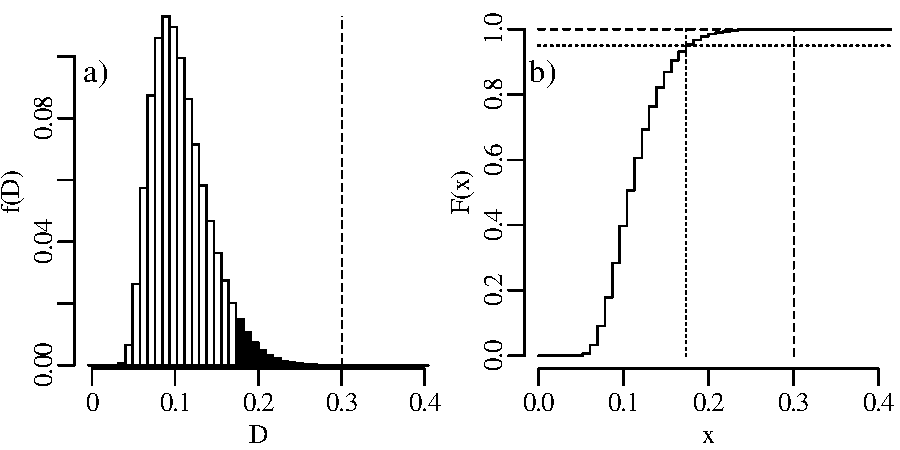
\includegraphics[width=\textwidth]{../figures/KSdens.pdf}\medskip
\end{minipage}
\begin{minipage}[t][][t]{.4\textwidth}
  \captionof{figure}{a) PMF and b) CDF of the Kolmogorov-Smirnov
    statistic for comparison of two samples containing 116 and 121
    items, respectively.  The vertical dashed lines mark the test
    statistic for the two sand samples of Figure~\ref{fig:KS}. The
    rejection region is marked in black on the PMF and groups all
    values of the test statistic that exceed the 95 percentile
    ($D=0.174$).  $H_0$ is rejected.}
  \label{fig:KSdens}
\end{minipage}

The Kolmogorov-Smirnov test can not only be used to compare two
samples with each other, but also to compare one sample with a
theoretical distribution. Here, for the sake of illustration, we
compare the dune sample with a normal distribution that has the same
mean and standard deviation:

\noindent\begin{minipage}[t][][b]{.35\textwidth}
  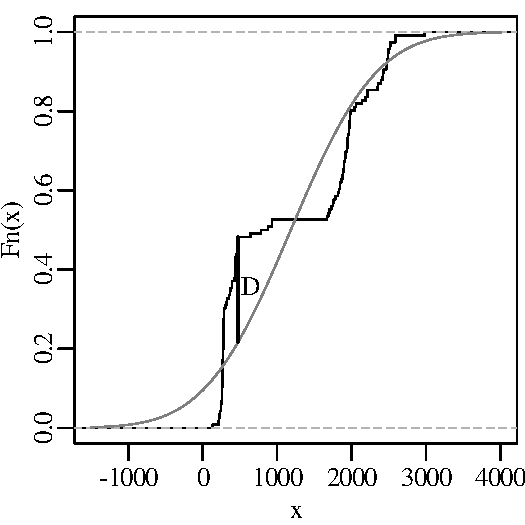
\includegraphics[width=\textwidth]{../figures/KSnorm.pdf}\medskip
\end{minipage}
\begin{minipage}[t][][t]{.65\textwidth}
  \captionof{figure}{Kolmogorov-Smirnov statistic for the comparison
    of a sample with the normal distribution with the same mean and
    standard deviation. In this case $D=0.27$, which can be compared
    with a lookup table for a \textit{one sample} Kolmogorov-Smirnov
    test. The outcome of this test (which is not elaborated in these
    notes) is a rejection of the null hypothesis.}
  \label{fig:KSnorm}
\end{minipage}
